\chapter{Sun City}

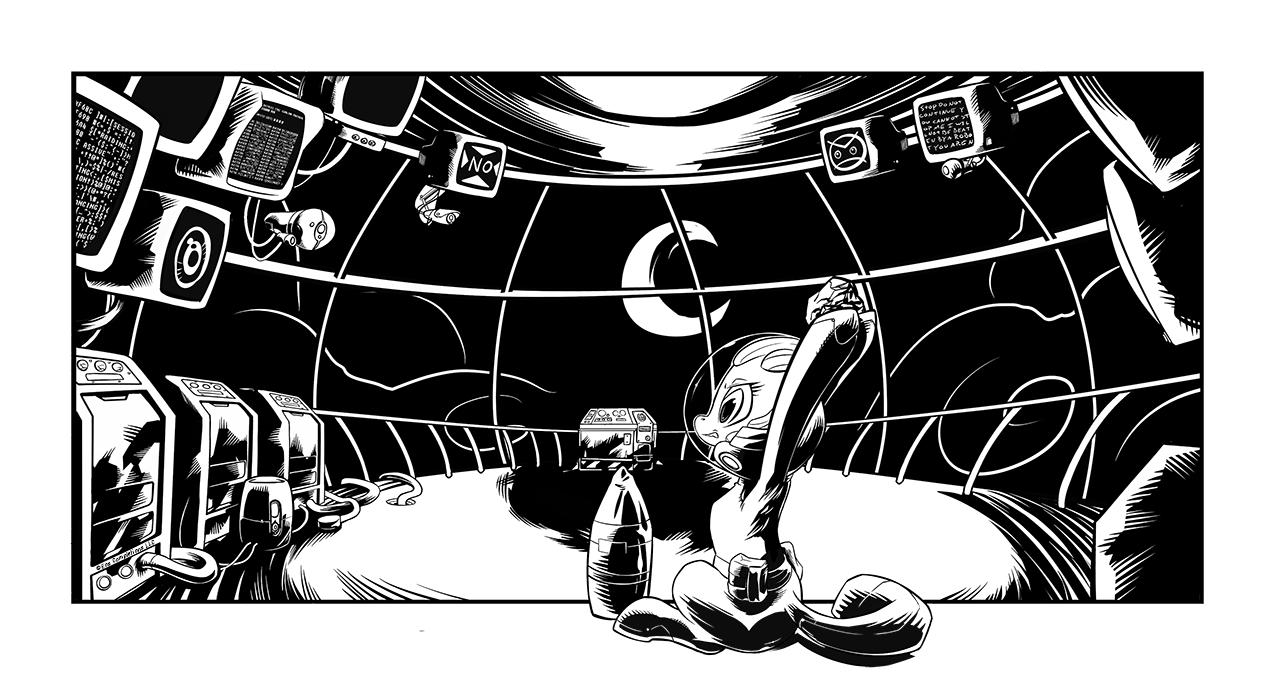
\includegraphics[width=\linewidth]{image09.png}


\begin{intro}
    Sun City is more than a town: it's the remedy to ponykind's derailment.
\end{intro}

\englishdaytimeplace{7}{11:00 P.M.}{Sun City Suburbs, Big 52 SC Branch}

The trip to the city had been quite long and by the time Puppy arrived at the first houses darkness had already descended on the streets. Sun City featured a central group of commercial and administrative buildings surrounded by residential areas. However there were no lights in any window, nor signs of anypony living there. The neighborhood Puppy was trotting through had been almost completely scavenged for construction material, leaving only the skeletons of houses resting in the ever present sand; it was like a desolate boneyard, filled with carcasses that had once been called `home'.

Now, Puppy wasn't eager to admit that she still was a little afraid of the dark, but the whole place was a little too similar to her first day in the apocalypse to let her just shrug it off and keep going. ``Why that chicken had to be in danger in such a scary place? Stoopid Henri, there's nopony here, why they call it a city if it's empty?''

Each step took her deeper into that scary place. Where did the colorful signs go? Puppy never went out very much at night but she was pretty sure that a city didn't work like this\dots She wanted some music to hide the sound of the wind howling through those bony houses, but the radio had gone mute when the filly reached Sun City's outskirts and the unusual silence made her feel lonely. ``Hey, mister Voice, you there?''

A discharge of static was the only answer Puppy got from the suit. ``{\mt Fzzt -cation BbZzzZzT -ched. Elctr- SkrackLE -ference. BzaP! -sible sustaining vo- BzZzT! -terface.}''

``Aw, he's grumpy again\dots'' The filly frowned and kept trotting. The HUD of the helmet started to display written warnings on the screen, but showing fast scrolling technical messages to a foal that couldn't even read without spelling every single letter was a waste of time. This left the filly completely alone: the radio was gone, mister Voice was gone, this was like those times when she tried to sleep but the room was too dark and the wind outside made strange noises. They were the nights when she'd hid under the sheets and called out for her mother until she came and nuzzled her, singing a little lullaby to make her feel safe and warm. Puppy actually tried to sing something, but the only thing she could think of right now was the evil enchantress song and no, it didn't help at all.

The little pony's steps echoed in her head like the beat of drums as Puppy walked through a never ending maze of identical streets, with every empty window reflecting her eerie pink glow. What was that? Maybe mister Horse Tile came back from the grave and was following her? Even mister Horse Tile would have been welcome at this point\dots A distant metallic screech froze the filly in the place; her rump hit the asphalt and she completely stopped moving.

``W-w-whatwasthat!?'' Sure, dealing with bullybots and running after mom was not a frightening thing, having to face ghoulie ponies could be scary but at least you knew what you were fighting\dots but this one was different: an empty town filled with empty houses and crisscrossed by empty roads during a clouded night? And with ghostly sounds too? Why did she think about ghosts now? No ghosts, bad ghosts! Why did she leave the red banner trail? Miss pretty pony Happy told her not to leave the trail, but she had to come and help that stoopid chicken and now it was dark and it was scary and Puppy missed Miss Silky Tail so much!

The filly flattened herself against the road and lowered her ears, trying to make herself disappear. ``N-new plan, we wait here till it's day!''

Another creak echoed in the empty streets, like the suffering wail of a tortured soul.

``EEEEEEK!'' Puppy jumped on all four hooves and started galloping faster than Rainbow Dash at the Running of the Leaves. ``Newest plan! We're out of here till it's day!''

\begin{center}
Sun City 1 -- Puppy 0    
\end{center}

\horizonline

\englishdaytimeplace{8}{8:00 A.M.}{Sun City, Big 52 SC Branch}

During the day, the city was quite similar to the suburbs of Salt Cube City, or even Canterlot; not scary at all, just\dots ugly; Puppy wondered why she had been so scared, what a silly pony she was!

``See, mister Voice? There's nothing to be afraid! It's just another town, with broken houses and broken roads and-'' For a moment Puppy's eyes caught the silhouette of a flying pony, ``and pretty peggysuses! Yay!''

The foal launched herself into a gallop, chasing the flying figure. ``Hey! Hey mistur peggysus wait for me! WAAAAAIT!'' Galloping at top speed while looking into the sky, Puppy wasn't properly watching the road in front of her and collided with another pony in the middle of the street. ``Owie, why don't you look where you're going? I was running here before you!''

The pony was an adult earth stallion with a brown coat and black mane; he had been carrying buckets full of bricks and building materials on his back, but now everything was scattered over the asphalt. Puppy jumped onto her hooves ready to zoom away just in case the older pony was mad at her, but he simply put down the buckets and started filling them again.

``Uh, yeah, you better say nothing\dots and don't stay in the middle of the road again like a dumb statue!'' Puppy stuck out her tongue, but noticed that the earth pony wasn't even paying attention to her. Actually, he seemed a bit\dots well, how to put it\dots

``Ah, sorry mister pony, are you deaf? I'm Puppysmiles and I'm looking for my mom\dots well, usually I do that but today I'm saving my friend Henry that came here and then had some sort of troubles but I still don't know what kind of troubles. Have you seen her? She's a chicken but she doesn't want me to call her that way but I mean, duh, she has a beak and feathers and everything else, she must totally be a chicken. Once I knew a pony that was a zebra, I don't know why ponies don't like zebras, anyhow this zebra didn't want to be called zebra but everypony called her that all the same, so maybe she's just like zebras, maybe ponies don't like chickens here\dots dunno\dots''

Puppy followed behind the earth pony as he, without saying a word, gathered everything that he had dropped and headed toward the center of the city. In the light of day, Puppy could see that past the outer town borders the houses had been completely dismantled, leaving a vast area of flat terrain traversed by an intricate web of paved streets in a ring of at least two hundred meters all around downtown. It seemed like some sort of nopony's land, but it was the result of the methodical demolition of every building that had stood in the area, brick by brick instead of simply flattening the houses. They weren't even using the ruins as defensive positions; the buildings had been salvaged down to their foundations.

Puppy stopped and gazed in wonder at the shining city that lay at the heart of the empty land. ``Wow, you have a pretty town here at last, I like it!''

Right in front of the filly in yellow stood a city of the old times: there were some small houses with painted walls and clean windows, no holes in their roofs nor planks nailed over the doors. Puppysmiles stared at the ponies trotting around and carrying things, it was a lively place: everypony was doing something, even the foals and the pegasi. There were pretty houses and pretty skyscrapers; even if the gardens were a little yellowish there was actual grass in the yards and there were even trees here and there. Puppy wouldn't have given this place more than a six out of ten, but hey, this was the first town along her way that deserved a vote at all!

``Really, Happy was super wrong\dots'' Puppy trotted after the brown pony she had bumped into earlier, ''ponies that arrived here actually liked it so much that they didn't want to leave! I was right as usual, ah, take this miss Happy! Sure you aren't very chatty mister pretty pony\dots'' Nope, not chatty at all, Puppy decided to leave the earth pony and wander by herself so she could check the place out. It was really a nice town and reminded her of some of rhe places she had visited with her mom: after eight days of wasteland being in such a nice place was refreshing, even if these ponies had something wrong with them that Puppy couldn't put her hoof on.

The filly in yellow searched the area for some other pony to talk to, and noticed a griffon crouched on a roof; he was replacing some damaged tiles. ``Hey mister chicken, have you seen my friend Henri? She' a chicken too!'' Nope, no answer at all; in this place everypony had to be deaf or really unfriendly.

Puppy saw a unicorn mare watering a tree, and tried to approach. ``Ah, excuse me miss pretty pony, have you seen a chicken named Henrietta please?'' Nothing again, the filly's frustration was growing; it was quite obvious that she was getting nowhere, this situation needed something better: ``Uh, she's half kitty too.''

The unicorn kept watering the tree despite Puppy's efforts, but this time the filly wasn't going to give up that easily: she put herself physically between the tree and the unicorn, staring her right in the eyes and\dots and\dots DERP! ``Ah, your eyes are\dots uh, weird\dots''

The mare had a walleyed expression and seemed frankly dumb. ``How do you make that trick with the eyes?'' Puppy tried crossing her eyes and almost fell on her rump, ``It's hard! How can you look straight with eyes like that?''

Again, the foal was completely ignored. The mare tried to circle around Puppy a couple of times, but the filly in yellow insisted on staying between the unicorn and her tree; in the end she watered Puppy's head and went away.

Puppy was now wet and upset. ``Hey, that's not very nice! What's up with everypony here? Why don't they want to talk with me, do I stink?'' The filly tried sniffing herself but it was quite pointless since she was sealed inside the suit.

The foal wandered through the neighborhood for half the morning, trying to find somepony who would talk to her, but everywhere it was the same: everypony had the same walleyed expression and didn't listen to her, not even the ghoulies.

She could remember something like this, a movie with a strange title that her mom forbid her to watch, metrodontremember\dots anyhow she tried looking it but it was boring to death. This city was just the same: like a warped reflection of the barns of horrors where fun could actually kill you, here the boredom could turn you to stone.

Her exploration took the filly deeper inside the town and nopony tried to stop her or seemed to acknowledge her passing Even when Puppy approached some foals trying to play with them, they simply kept working; she really did her best to make some friends, proposing some games like pin the tail on the pony and even something exotic, like playing space ponies and the tomato aliens, but nothing. Now she was feeling ignored and a bit sad.

``Mister Voice has gone away, Henri is nowhere to be seen and all the pretty ponies play dumb and don't want to talk with me. This is the worst city ever! Who cares about the pretty houses or the nice trees if there is no fun at all in first place? Why is everypony acting this weird?'' Puppy sighed; she knew for a fact that in each town there was at least a mayor or something like that, maybe she could find some answer if she asked that pony. Usually important ponies lived in the middle of town and this was quite good, because finding the center of Sun City was easy even for a silly pony: those giant skyscrapers were quite hard to miss.

The little foal trotted past the residential area and arrived in a wonderful and well kept block of tall buildings, with glass walls and picturesque statues of Celestia and Luna. Around the marble princesses were fountains that spilled clean water, and a big metal tower stood right in the middle of everything, like a focal point for the whole city. Puppy lifted her head as she looked around at the various buildings: there were half a dozen towers of various heights, but one of them stood out because of it's shiny metallic structure; it was like a spiral growing into the sky for about twenty stories and then abruptly ending in a large platform, like an overgrown mushroom.

``This one seems easy!'' Puppy trotted toward the tower only to find herself being lifted off the ground and floated away from her destination. ``Wut?'' The foal tried to twist around and saw that an adult pony had picked her up by the back of her neck and was taking her away toward the residential area.

``Hey! Lemme go! Meany pony I wanna go to the shiny tower! I gotta see the mayor! It's important, you dumb walleyed pony, are you listening to me?'' The pony put Puppy down just outside of the city's borders in nopony's land, leaving the protesting foal still yelling at him.


\begin{center}
    Sun City 2 -- Puppy 0
\end{center}

\horizonline

\englishdaytimeplace{8}{2:00 P.M.}{Sun City, Big 52 SC Branch}

Puppy spied on the working ponies with a resolute look on her face: they didn't want her in town and wouldn't tell her why, but she had to get inside somehow\dots maybe she needed to play smart, with some sort of disguise using a sombrero and a poncho and maybe an accordion\dots yeah, that could actually work, but where to find fake mustache at this hour?

Suddenly, the filly was distracted by another flying figure in the sky. She had grown used to pegasi flying to and fro around the outer part of the city, but this one was different: it was a griffon, a little griffon with familiar armor\dots ``Henry! Hey Henri, wait!'' Nope, even her best of bestest friends wasn't listening to her now; Puppy would have felt disheartened if she wasn't busy finding a way to get Henrietta's attention, ``Rock!''

\emph{The Rock Of Destiny} floated to Puppy's hoof, she took a moment to aim aaand\dots ``Bull's eye!'' The griffon unleashed a panicked screech as she dropped out of the sky like, well, the rock that hit her.

``Don't worry I'm catching you Henri!'' Puppy threw herself into a gallop, trying to catch her feathered friend before she hit the ground. In the meantime Henrietta struggled desperately to regain control, but she was still stunned: all she could do was to try and aim for something soft\dots but what? A yellow spot appeared in her peripheral vision. A yellow spot that was yelling and moving fast.

``I got you I got you I got-''

THUMP! ``Owie!'' ``Yeow!''

The young griffon blinked, looking at Puppysmiles. ``What the fuck are you doing here, Puppy? This place is dangerous, run! There's a strange buzz tha-'' Henrietta derped and immediately stopped talking; a trickle of blood from her head injury ran down her beak but she didn't even seem to notice.

``Henry I found you at last! Silky Tail told me that you were in danger and- HEY! Where do you think you're going!?'' The griffon opened her wings, getting ready to take-off, but the filly wrapped her hooves around Henry's neck and held on tightly. ``Don't even think of going away! Now we are getting out of this stoopid place and you are coming with meeEEEH!''

Henrietta was bigger and stronger than Puppy, and she seemingly felt no remorse in using brute force to push her away before taking to the air once again; the filly rolled head-over-heels a couple of times before finding herself sitting in a pile of rubble in nopony's land, alone once again.

``What the\dots what happened to her all of a sudden? The other day she was all let's work together and then she was wounded and I helped her and now she just scolds me and flies away\dots this is not fair, not fair at all! Very well, if she doesn't want to be my friend, then I want Silky Tail back!'' Puppy galloped back into town, looking for her ex-friend, but almost immediately came to a stop and reconsidered her last thought, ``But I gave her Silky as a present, I can't take a present back\dots but I want back my friends, at least one of them.''

Puppy shook her head. ``No, I want both of them back! I'm not going away without Henri AND Silky Tail! I only need a better plan!'' But what plan? During the day the ponies were all around the place and didn't let her walk into town and during the night the city was so scary\dots or maybe not? After all, this wasn't a ghost city\dots

The foal went back to sitting just outside of the town borders and looking at the not-really pretty ponies working endlessly and mindlessly. She had come up with a masterful plan\dots now she just had to recover The Rock Of Destiny and wait for night\dots Half hidden behind a pile of rubble, Puppy lurked, ready for the decisive strike. ``Soon\dots''


\begin{center}
    Sun City 3 -- Puppy 0
\end{center}

\horizonline

\englishdaytimeplace{8}{9:00 P.M.}{Sun City Downtown, Big 52 SC Branch}

The little filly crept through the dark, crawling with her belly on the ground and her ears flattened. ``Sneaky sneaky\dots'' She uttered a couple of whispered words, nothing more: like those oriental ponies who did all that cool stuff she was told about but she had never actually seen because mom said they were violent\dots sometimes mom was a pain. But none of that mattered because now Puppy was a filly on a mission, and she had to focus and be super sneaky and move like a shadow in the night!

Wearing a yellow suit and a pink glowing fishbowl. ``Sneaky sneaky\dots''

The plan was easy: go past the enemy lines, find the boss of the place, tell him his town stinks then go find Henri and run away in the sunset, like in that super cool movie with Pone Wayne. Now, first things first: poke her nose into the super pretty place with the skyscrapers and have at least one ride on the elevator. Okay let's get real: ride the elevator until it melts.

The city was completely empty during the night: everypony was somewhere else, probably sleeping, but this time Puppy knew that there were no ghosts in this place, only grumpy faces. Reaching downtown had been an easy task and nopony blocked her when she ventured deeper into the heart of Sun City. It was as if somepony had built a brand new town ready for the use and moved away leaving everything behind. The filly had never actually seen a brand new city, but she supposed that when you unpacked a new one it would look just like this.

The only place where Puppy could see some light was the mushroom tower: a faint blue glow came from the black windows while the upper part of the tower sometimes crackled with an electrical bolt. A faint humming sound came from the metallic structure, like the one that comes from some big electrical stuff that mom didn't want her to touch because it was really, really dangerous \py{\dots and when I say it I mean it Puppy! Are you paying attention Puppy? Look at me and repeat what I say: this is not a toy and I will never ever ever touch it!}

``Sneaky sneaky\dots''

Cautious exploration of the area surrounding the tower revealed a closed entrance and no open windows. On the dark glass doors was depicted the symbol of Solaris Inc; Puppy tried to push the door, then pull it, then ram it and finally, to yell at it: ``Hey, how am I supposed to sneak inside this place if there is no way to get in? Stoopid tower, why you don't co-operate? I am the hero here, don't you know?'' As usual Puppy had to do everything by herself: this was the price of being surrounded by amateurs.

``Rock.''

It was a glass door: whenever the filly had played with a ball in the neighborhood, breaking windows was apparently a thing that happened even if you didn't want it to happen, so if you actually wanted to break a glass then it had to be a piece of cake; obviously Puppy never heard of bulletproof glass, so it took a little more than she thought it would.

When the glass of the door finally gave up, detaching itself from the door's frame, Puppy took a long pause admiring her work: this glass was similar to the one used in her helmet, cracking and changing its shape rather than simply falling down, so that a couple of good placed hits were far from pulling the trick; luckily enough the foal had learned how to use a stone from her previous experiences, refusing to give up at the first difficulties and thus being rewarded with a hole trough the door after half an hour of hitting and cursing against a glass panel.

The filly was still panting when she stepped inside the building, but at this point she was so excited by her new adventure that she simply couldn't help giggling, and with the giggle she began singing.

\begin{song}
you better watch out, you better not cry

you better not pout, 'cause I'm telling you why:

Puppysmiles is coming to town.
\end{song}

It's unlikely that anypony was listening at that time in that place, but the filly felt as if it had to be done: after all she was going to scold the bad mayor of a bad town, he'd better know what was coming for him!

When the foal reached a large desk in the middle of the hall, a red light started to flash from the ceiling and an automated voice began to talk. ``{\mt Warning: unauthorized drone presence in reception, all personnel please stay in their offices, security will take care of the emergency.}''

Puppy had no idea what a reception or a drone were, but she already knew the meaning of that lullaby: bullybots incoming. ``Hey, don't even try bullying me, I have a rock! Got it?'' The filly showed her favored weapon to nopony in particular and trotted past the desk. A couple of turrets popped up from two big floor tiles and opened fire, but the only sound they made was that of empty magazines. Puppy looked at the turrets with a puzzled expression, trotted towards the nearest and poked it with a hoof.

``Yeah, you better behave!'' The filly stuck out her tongue and headed for the elevator, but it had a red light and didn't want to go anywhere, her usual luck\dots she had to hit the stairs but this didn't prevent her from singing.


\begin{song}
She's making a list and checking it twice,

she's gonna find out who's naughty and nice,

Puppysmiles is coming to town.
\end{song}

The stairs were quite long and went past a lot of identical floors all filled with clean, empty rooms, as if they were ready to receive furniture that had never arrived.

At the top of the stairs was a reinforced door, once again decorated with the company's logo. Puppy knocked at it with a hoof, ``Hey, I'm Puppysmiles and I want to see the mayor! This town stinks!'' When she didn't get a reply she hit the door again and yelled louder, ``Don't ignore me! Everypony is ignoring me in this lousy place, even my bestest friend ever! Even mister Voice! Why you don't want to make friends?''

Still nothing, but Puppy knew that the mayor was there: everypony knew that the mayor lived in the town hall and now it was night so he had to be there because he was sleeping. This time the foal wasn't going to give up: she still had that thingy Sand Box gave her, that strange remote control that opened doors just pressing a button. ``Things that opens doors!'' Puppy raised a hoof as a bobby pin and a screwdriver floated out in front of her; the filly looked at the objects with disapproval. ``How am I supposed to open a door with these things!? The other one, with the big black button, the red cables and the blue screen!''

Sand Box's hacking tool floated in front of Puppy, who gave a nod and grabbed it out of the air before looking at the door with her best menacing face. ``Very well mister: I have a\dots thing that can open this door lickety split and you are gonna open it or I'll do it and if I have to do that I will be very, very dis- daisy pointed!'' When mom was really, really angry she used that super scary ultimatum and Puppy knew that after that there was the spanking, so she was sure that this one was going to work.

The door resisted her threats. ``Okie dokie, let's do this the hard way\dots'' Puppy sighed and pressed the button on the hacking tool; the screen fizzled and started showing a cascade of numbers while a small vent behind it made a whistling noise; the screen flickered and crackled before turning green and almost immediately died with a small puff of smoke, but the door opened. ``See? I told you so!'' The foal jumped inside the room and faced-

A couple of skeletons? ``Hey but there's nopony here!'' The large room was very similar to the control room of the Dome, but it was circular and had windows all around its perimeter so that it was possible to see the whole city from here. There were several desks with computer terminals and a big screen just in front of the door; all the screens were lit, glowing with a dim blue light. The only sign of pony presence in the room was the pair of skeletons lying on the floor immediately in front of the door, nope, skellies weren't very scary\dots

Suddenly a deep manly voice started talking out of nowhere. ``There is nothing here for you Device 018, now go away.''

The filly was confused and looked around for the source of the voice. ``Wut? Where is the mayor?''

The voice replied with a neutral tone: ``There is no mayor: she died nineteen years ago and I have been taking care of Sun City since then. This is no place for you, don't test my patience.''

Puppy noticed the big screen's blue light blinked as the voice spoke. ``Oh, another voice! But a voice can't be the mayor of a town, sillybot! uh\dots I already know a mister Voice, so I'll call you Blue Voice!''

This time the voice boomed like angry thunder. ``You are not meant to name things and certainly not me, useless malfunctioning machine! I am SolOS and I am the master of Sun City. Besides, voices have no color.''

Puppy waved a hoof dismissing the last piece of information. ``Whatever; I'm Puppysmiles and I was looking for the pony in charge because his town is ugly and I want my friends back.''

``I already told you that there is no pony in charge here! I command this place, I am the boss! Mr Number One! And if you think that this place is `ugly', listen to this! Before I arrived this place was a war zone, with ponies killing each other and every sort of depravity performed in broad daylight! There were no sewers, the houses were a disaster and ponies would die even for something as simple as giving birth to a new foal! Sun City was meant to be the best city ever, the eternal symbol of Solaris' superiority over Stable Tech and their lackeys! Do you have the slightest idea of the work that was needed to clean the radiation and build a half decent barrier around the place to break the desert winds? Now Sun City is a jewel, the last shining ruby in a rusted crown, but it still stands and I did that! Ponies proliferate under my guidance, maybe they were deprived of their free will but look at what they did when they had the power to choose their destiny! It was ME that saved this place when it was falling apart, ME that rebuilt it from its foundations and ME that saved hundreds of pony lives by forcing them to collaborate and live in harmony and peace! Now you, a puny little crazed machine, come here, break into my control room and treat me like a common computer only to tell me that you don't like the place!? You are nothing but a-''

Puppy snorted ``Boo-ring!''

``You are a waste of time, stop being irrational and go away immediately!''

Puppy giggled. ``Tee-hee, Blue Voice is funny when he's mad!''

``ENOUGH! I have no time to spare for a broken piece of equipment. Go away.''

``Ah, did you break something? Can I help you?'' Puppy tilted her head, a bit confused.

``No, stupid low level Artificial Intelligence, YOU are the broken machine!''

Puppy giggled again. ``Silly Voice, I am a pony, you are a machine! Machines are stoopid!''

``{\mt Negative, you are FES MK-VI device 018: a piece of equipment meant for preserving the life of a pony in a hostile environment, fitted with a basic Artificial Intelligence capable of making simple decisions in case of extreme danger. From what my scanning modules can tell, you utterly failed your purpose and now you believe that you are the pony that you failed to protect: a female earth pony named Puppysmiles.}''

Puppy tilted her head, smiling. ``Blue Voice says funny words! What is an envy room mate?''

The voice paused for half a minute and when it came back it had resumed its original neutral tone: ``Alright, you want this the hard way? You are not a pony, you are a robot. Now go away and cope with it. You're not worth my time nor my pity.''

This time the filly frowned and took a couple of steps back. ``I am not a robot, I am Puppysmiles!''

``No you are not!''

``Yes I am!'' insisted the little pony.

``No you are not!''

``YES I AM!'' Puppy screamed.

``No. You. Are. Not!''

``YES! I! AM!'' Pink flames flared inside the helmet.

``YES YOU ARE!''

``NO! I'M! NOT!'' Puppy frowned as soon as she realized that the voice had tricked her. ``Hey!''

``Gotcha.'' If it was actually possible for a computer screen to smile, SolOS would have been grinning from ear to ear. ``Now, since you don't want to go away, and I gave you the opportunity to do so, activate protocol ES-01 emergency shutdown and erase memory, command line A-0101101101 bypass codes using priority Easy, Gallop, Luna, 90670.''

Puppy blinked her eyes looking a bit puzzled at the blue screen talking nonsense. The suit started showing strange numbers everywhere and a big clock appeared in the middle of the HUD, but this wasn't what bothered her the most: the Voice made her seem a fool! ``I am not a robot and I'm not stoopid! You are stoopid and I'll show you!'' Puppy rose a hoof, ``Teapot!''

A large tank shell with a blue band round the top floated out of her inventory. Trigger didn't want this shell because she said that it was only dangerous for robots, so Puppy could keep it; the guard chief of Tunnel Town also explained to the foal how to use it: just pick something hard and hit on the teapot head until it goes 'FZAP!'.

``Don't complain, I gave you the opportunity to leave but you didn't want to listen and I have a city to administrate, you can blame only yourse-''

CLANK!

The sound of something hard striking metal distracted SolOS' monologue.

``What are you\dots that is a Mag Pulse 8.8 grenade! What are you doing, put that thing away it will disrupt every computer in the control room!''

Puppy was mad. Mad because he made her seem a fool; mad because he said she was a robot; mad because this city stole her best friend; mad because, and just because. ``Yeah, right! I'll put you to sleep for good, who's the silly pony now?''

CLANK!

``No, wait! You'll destroy the Behavior Control Center! The city will fall into chaos!''

Puppy was sitting on the floor in the middle of the control room, she didn't say anything and hit the tip of the shell with \emph{The Rock Of Destiny}. Yes, it was singing time again.

CLANK!

\begin{song}
    Who's a silly pony? You're a silly pony!

    Who is? You is, Puppysmiles!
\end{song}

CLANK!

``Stop it! Stop it now! If that charge detonates I won't be able to operate anything and will forever be locked inside the mane frame!''

The countdown was running on Puppy's HUD leaving her a single digit of seconds, but she couldn't read, so it wasn't her problem.


\begin{song}
Bumping into robots, knocking over ghoulies,

who is? You is, Puppysmiles!
\end{song}

CLANK!

``No wait! We can talk about this, you have no idea of what you are doing! This utopia will crumble without my guidance!''


\begin{song}
    All day long you trot around looking for your mommy everywhere,

    dreaming all your pony dreams, but you get lost every time!
\end{song}

``Okay okay you win! I am the silly pony but please sto-''

CLANK! FZAP!

There was something like an explosion, except that this one didn't launch Puppy to the other side of the room; a nice surprise for once. The countdown on the helmet disappeared, the whole HUD disappeared; actually, every screen inside the big room went black and the lights flickered for a moment before turning red and the Voice finally stopped talking. Ah! Who was the silly pony now, Blue Voice?

And why couldn't Puppy move at all, nor speak, or even blink her eyes?

She didn't feel pain and she didn't feel tired, nonetheless she couldn't move: all she could do was look around, like that time in Canterlot or at the Dome when for the first time she met miss Voice, but that time it was really short. This time it was different: there were no pink dots coming back to life on the HUD. Puppy waited for a while, but nothing happened and she lay sitting on the floor with an exploded tank projectile in front of her; the only thing she could do was sit and hope for\dots well, some miraculous rescuer.

Sitting alone in the red light made her recall SolOS' words; maybe she was a robot after all: that grenade was supposed to shut down only the bullybots but worked on her too; but Puppy couldn't be a bullybot\dots or she could? After all she wasn't a good pony: breaking things and disobeying mom was a bully thing. Mom\dots \emph{if I am a robot then is my mom really a mom or she is a robot too? I don't eat, don't drink and almost never feel sleepy, so maybe\dots but I don't want to be a robot, I want to be a pony! This is not fair, why that stoopid Blue Voice had to say those naughty things? I'm a pony\dots It's only that\dots I'm a pony\dots}

``\py{Yes you are, indeed. A beautiful, desperate pony\dots}''

A feminine voice echoed in Puppy's thoughts. This surprised the filly and scared her, who was talking?

``\py{Oh, right, introductions: I'm you, Puppysmiles. What a beautiful obsession you have, what a delicious innocence. You can't be a robot at all, trust me.}''

Yay\textasciitilde{} another voice\dots and she was also convinced that she was Puppysmiles. The filly was even more confused; but the new voice told the filly that she was no robot, so maybe she was a friend?

``\py{Listen to me little pony, because I will tell you only the honest truth: you are a pony; if you weren't, I couldn't even exist. We went through centuries of sleep and days of hunger and delusion, but now you have fallen and I must intervene: let me help you, open your eyes and you won't be a hermit crab in a cracked shell anymore.}''

Now Puppy was scared: this voice was talking weird and she wasn't even sure of what she wanted from her, but it felt wrong in a strange and itchy way:\dots

``\py{Simple minds are truly blessed. Pay attention: accept my help and you'll be out of this place and back on the road to finding your mother before the sun rises.}''

Maybe this was just a bad dream? Puppy had once dreamed of being unable to run very well or something like that, then she woke up all wrapped up in the sheets and mom arrived, hugging her and saying that she wasn't mad, even if she wet the bed and then everything was alright. Yes, just a bad dream, no Blue Voice telling her bad things and no ghostly voices scaring her in a dark dead room with the only company of two skeletons.

``\py{Oh silly pony, you are not having bad dreams, you ARE a bad dream, but with some more insight you could be better: with a resolve like yours and such an obsession and stubbornness, we could be a Nightmare!}''

Puppy wasn't sure that this new voice was trustworthy; it wasn't the usual 'don't talk with strangers' thing, it was more a deep sense of cold and sadness that emanated from it. Her instinct was screaming at her to not listen the newcomer, but\dots but\dots she was scared, and alone in the dark and the little pony wasn't even sure if she really was a pony at all. She wanted help, she NEEDED help: she wanted mister Voice back.

``\py{You are scared. It can't work if you don't accept me willingly, I can't help you as long as you won't open your eyes, but simple minds take time to accept new things. I'm going away, but soon we'll talk again and I'm sure that the next time you'll ask me to show you how to become\dots better. Until then take back your friend Mister Voice as a sign of good will.}''

A pink dot flickered on the HUD, immediately followed by a torrent of lines that flashed across Puppy's helmet while the internal software of the suit came back to life.

``{\mt Reboot complete. Checking version. Pink suite 7.0 lite. Checking equipment status. All systems online. Resuming last session. Loading personal data for subject 001: Puppysmiles. Subject deceased, condition stable. All clear.}''

~\vfill

\begin{engnote}
    Level up! (8)
    
    New perk added: Pack Rat - Wait a moment I think I have that! Carry weight is increased by 50 lbs.
    
    New Quest Perk added: Walking nightmare (rank 1) - there's something more than simple purpose in the way you keep pursuing your goals; you are now highly resistant to EMP grenades.
\end{engnote}


